\documentclass[letterpaper,12pt,]{article}

\usepackage[%
    left=1in,%
    right=1in,%
    top=1in,%
    bottom=1.0in,%
    paperheight=11in,%
    paperwidth=8.5in%
]{geometry}%

\usepackage{listings}
\usepackage{graphicx}
\usepackage{amsmath}
\usepackage[font=small,skip=-2pt]{caption}
\usepackage{subcaption}
\usepackage{hyperref}
\usepackage{booktabs}
\usepackage{pdfpages}
\usepackage{pgffor}
\usepackage[section]{placeins}


\lstdefinestyle{mystyle}{
    %backgroundcolor=\color{backcolour},
    %commentstyle=\color{codegreen},
    %keywordstyle=\color{magenta},
    %numberstyle=\tiny\color{codegray},
    %stringstyle=\color{codepurple},
    basicstyle=\footnotesize,
    breakatwhitespace=false,
    breaklines=true,
    captionpos=b,
    keepspaces=true,
    numbers=left,
    numberstyle=\footnotesize,
    stepnumber=1,
    numbersep=5pt,
    showspaces=false,
    showstringspaces=false,
    showtabs=false,
    tabsize=2,
    frame=single
}
\lstset{frame=single}

\pagestyle{empty} % Remove page numbering
\linespread{1.5} % Line Spacing

\begin{document}

\begin{titlepage}

\newcommand{\HRule}{\rule{\linewidth}{0.5mm}} % Defines a new command for the horizontal lines, change thickness here

\center % Center everything on the page
 
%----------------------------------------------------------------------------------------
%	HEADING SECTIONS
%----------------------------------------------------------------------------------------


\textsc{\LARGE McGill University}\\[3.5cm]
\textsc{\Large Computational Aerodynamics}\\[0.5cm] 
\textsc{\large MECH 539}\\[2.5cm]

%----------------------------------------------------------------------------------------
%	TITLE SECTION
%----------------------------------------------------------------------------------------

{ \huge \bfseries Project 2}\\[1.5cm] % Title of your document

\HRule \\[0.4cm]
%----------------------------------------------------------------------------------------
%	AUTHOR SECTION
%----------------------------------------------------------------------------------------

\begin{minipage}{0.4\textwidth}
\begin{flushleft} \large
\emph{Name:}\\
Doug \textsc{Shi-Dong} % Your name
\end{flushleft}
\end{minipage}
~
\begin{minipage}{0.4\textwidth}
\begin{flushright} \large
\emph{Student ID:} \\
260466662\\
\end{flushright}
\end{minipage}\\[4cm]

\vfill{}
{\large February 18, 2016}\\[2cm]

\end{titlepage}


\section*{Question 1}

\begin{figure}[!ht]
    \centering
    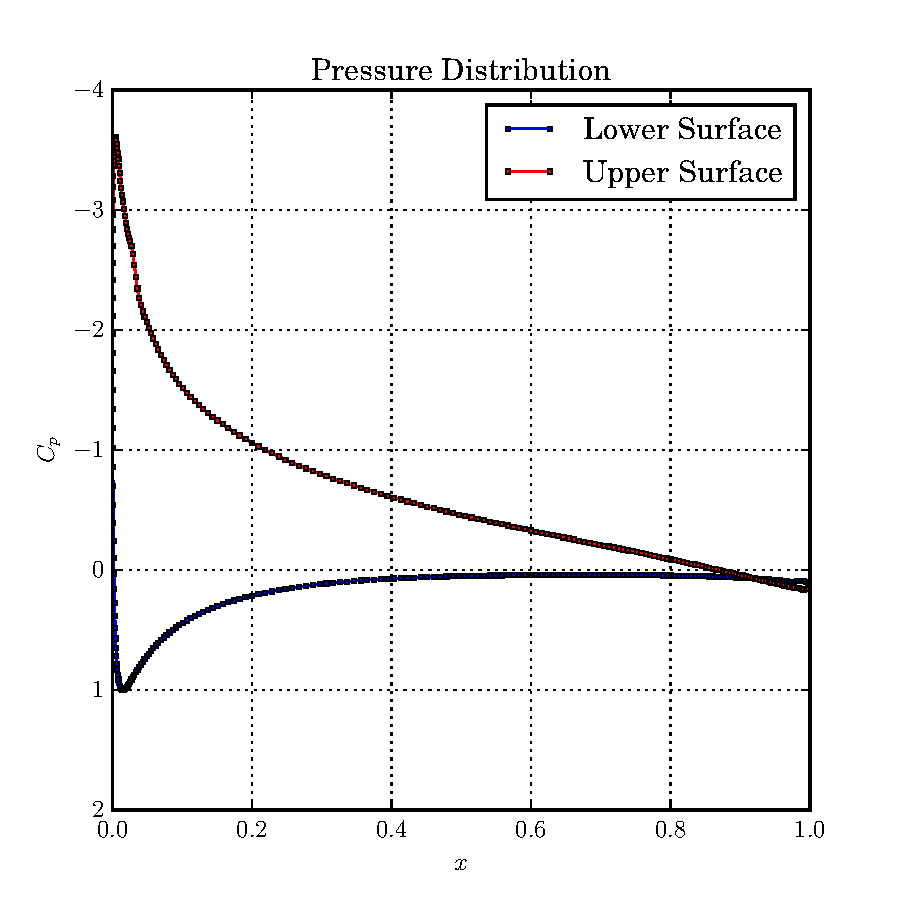
\includegraphics[width = 0.85\textwidth]{./Figures/q1.pdf}
    \caption {Surface Pressure Distribution}
    \label{fig:q1}
\end{figure}

\section*{Question 2}

\begin{figure}[!ht]
    \centering
    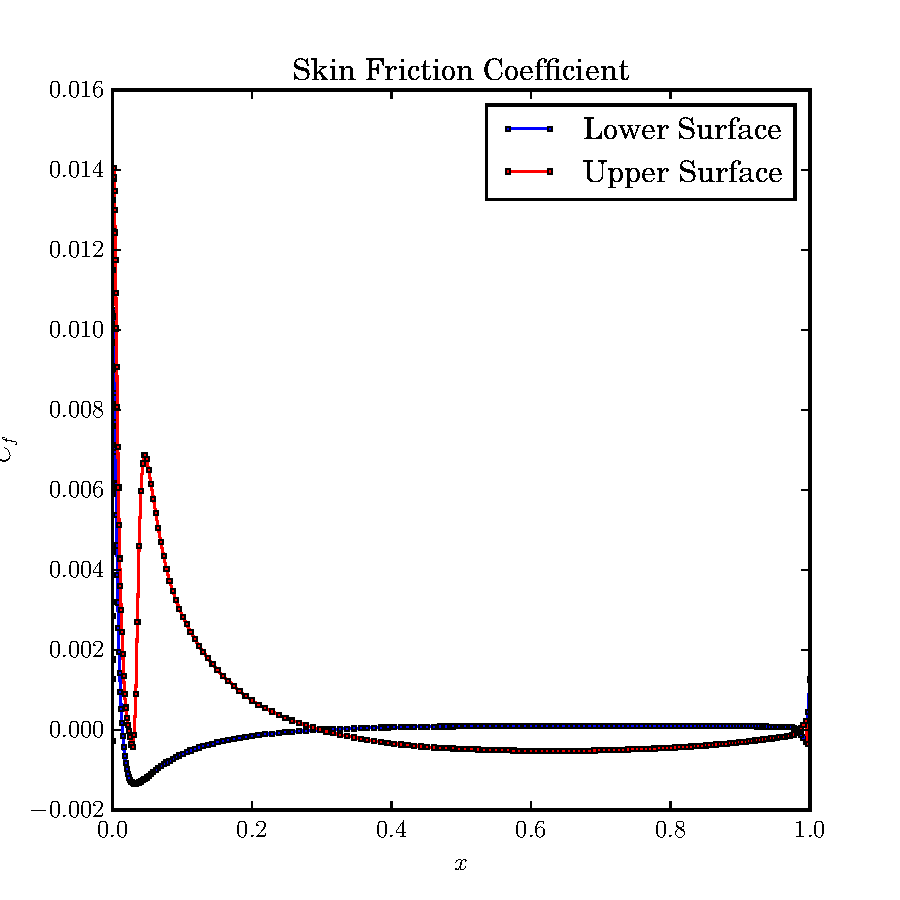
\includegraphics[width = 0.85\textwidth]{./Figures/q2.pdf}
    \caption {Skin Friction Coefficient Distribution}
    \label{fig:q1}
\end{figure}

\section*{Code}

Post-processing code has been written in Python available on my Github

\url{https://github.com/dougshidong/mech539/tree/master/a5}

\end{document}
